\chapter{Further Work}
\label{further_work}
%Nogle ideer til further work:
%videre arbejde - trådløs - mixer (midi/equalizer/garageband/sampling) - batteri (med beregning) - ergonomi -  processor (lav pcb med processer) - lydkort - hukommelse - interface (hvis ikke knapperne selv så en skærm) - placering af sensorer (håndfladen) - flere sensorer (kompas accell gps) - hovedetelefoner/højtaler m. forstærker. - To handsker + fødder -    

The finger drums prototype is in its current state, dependent of long wires connecting the FSR's to the Arduino, and the arduino to the computer. One of the most obvious improvements for the prototype, would be to make it wireless. This however requires a number of additions. Firstly the computer running the system should be located on the users body. This could be either a smartphone or maybe in form of a small integrated computer, similar to \autoref{fig:DisplayGlove} . Regardless some form of wireless communication is needed to avoid the long wires running along the body of the user. The computer should be able to contain the music files and therefore should have a form of storage unit, like an micro SD card for saving the files. For running a computer without an external power source, a battery is required which could be a form of LiPo battery that is rechargeable so that the user doesn't have to change battery. For playing the sounds both a soundcard and a speaker or a set of headphones is required to play the music, either out loud or in private. This would make a bluetooth module an ideal addition to facilitate communication with a phone or wireless headset.
If the prototype is connected to a screened device like a smartphone, interactions like changing drum kits and adjusting volume and sensitivity, as well as the storage of soundfiles etc. could be moved there to save on power consumption and manufacturing cost.

\begin{figure}[H]
\centering
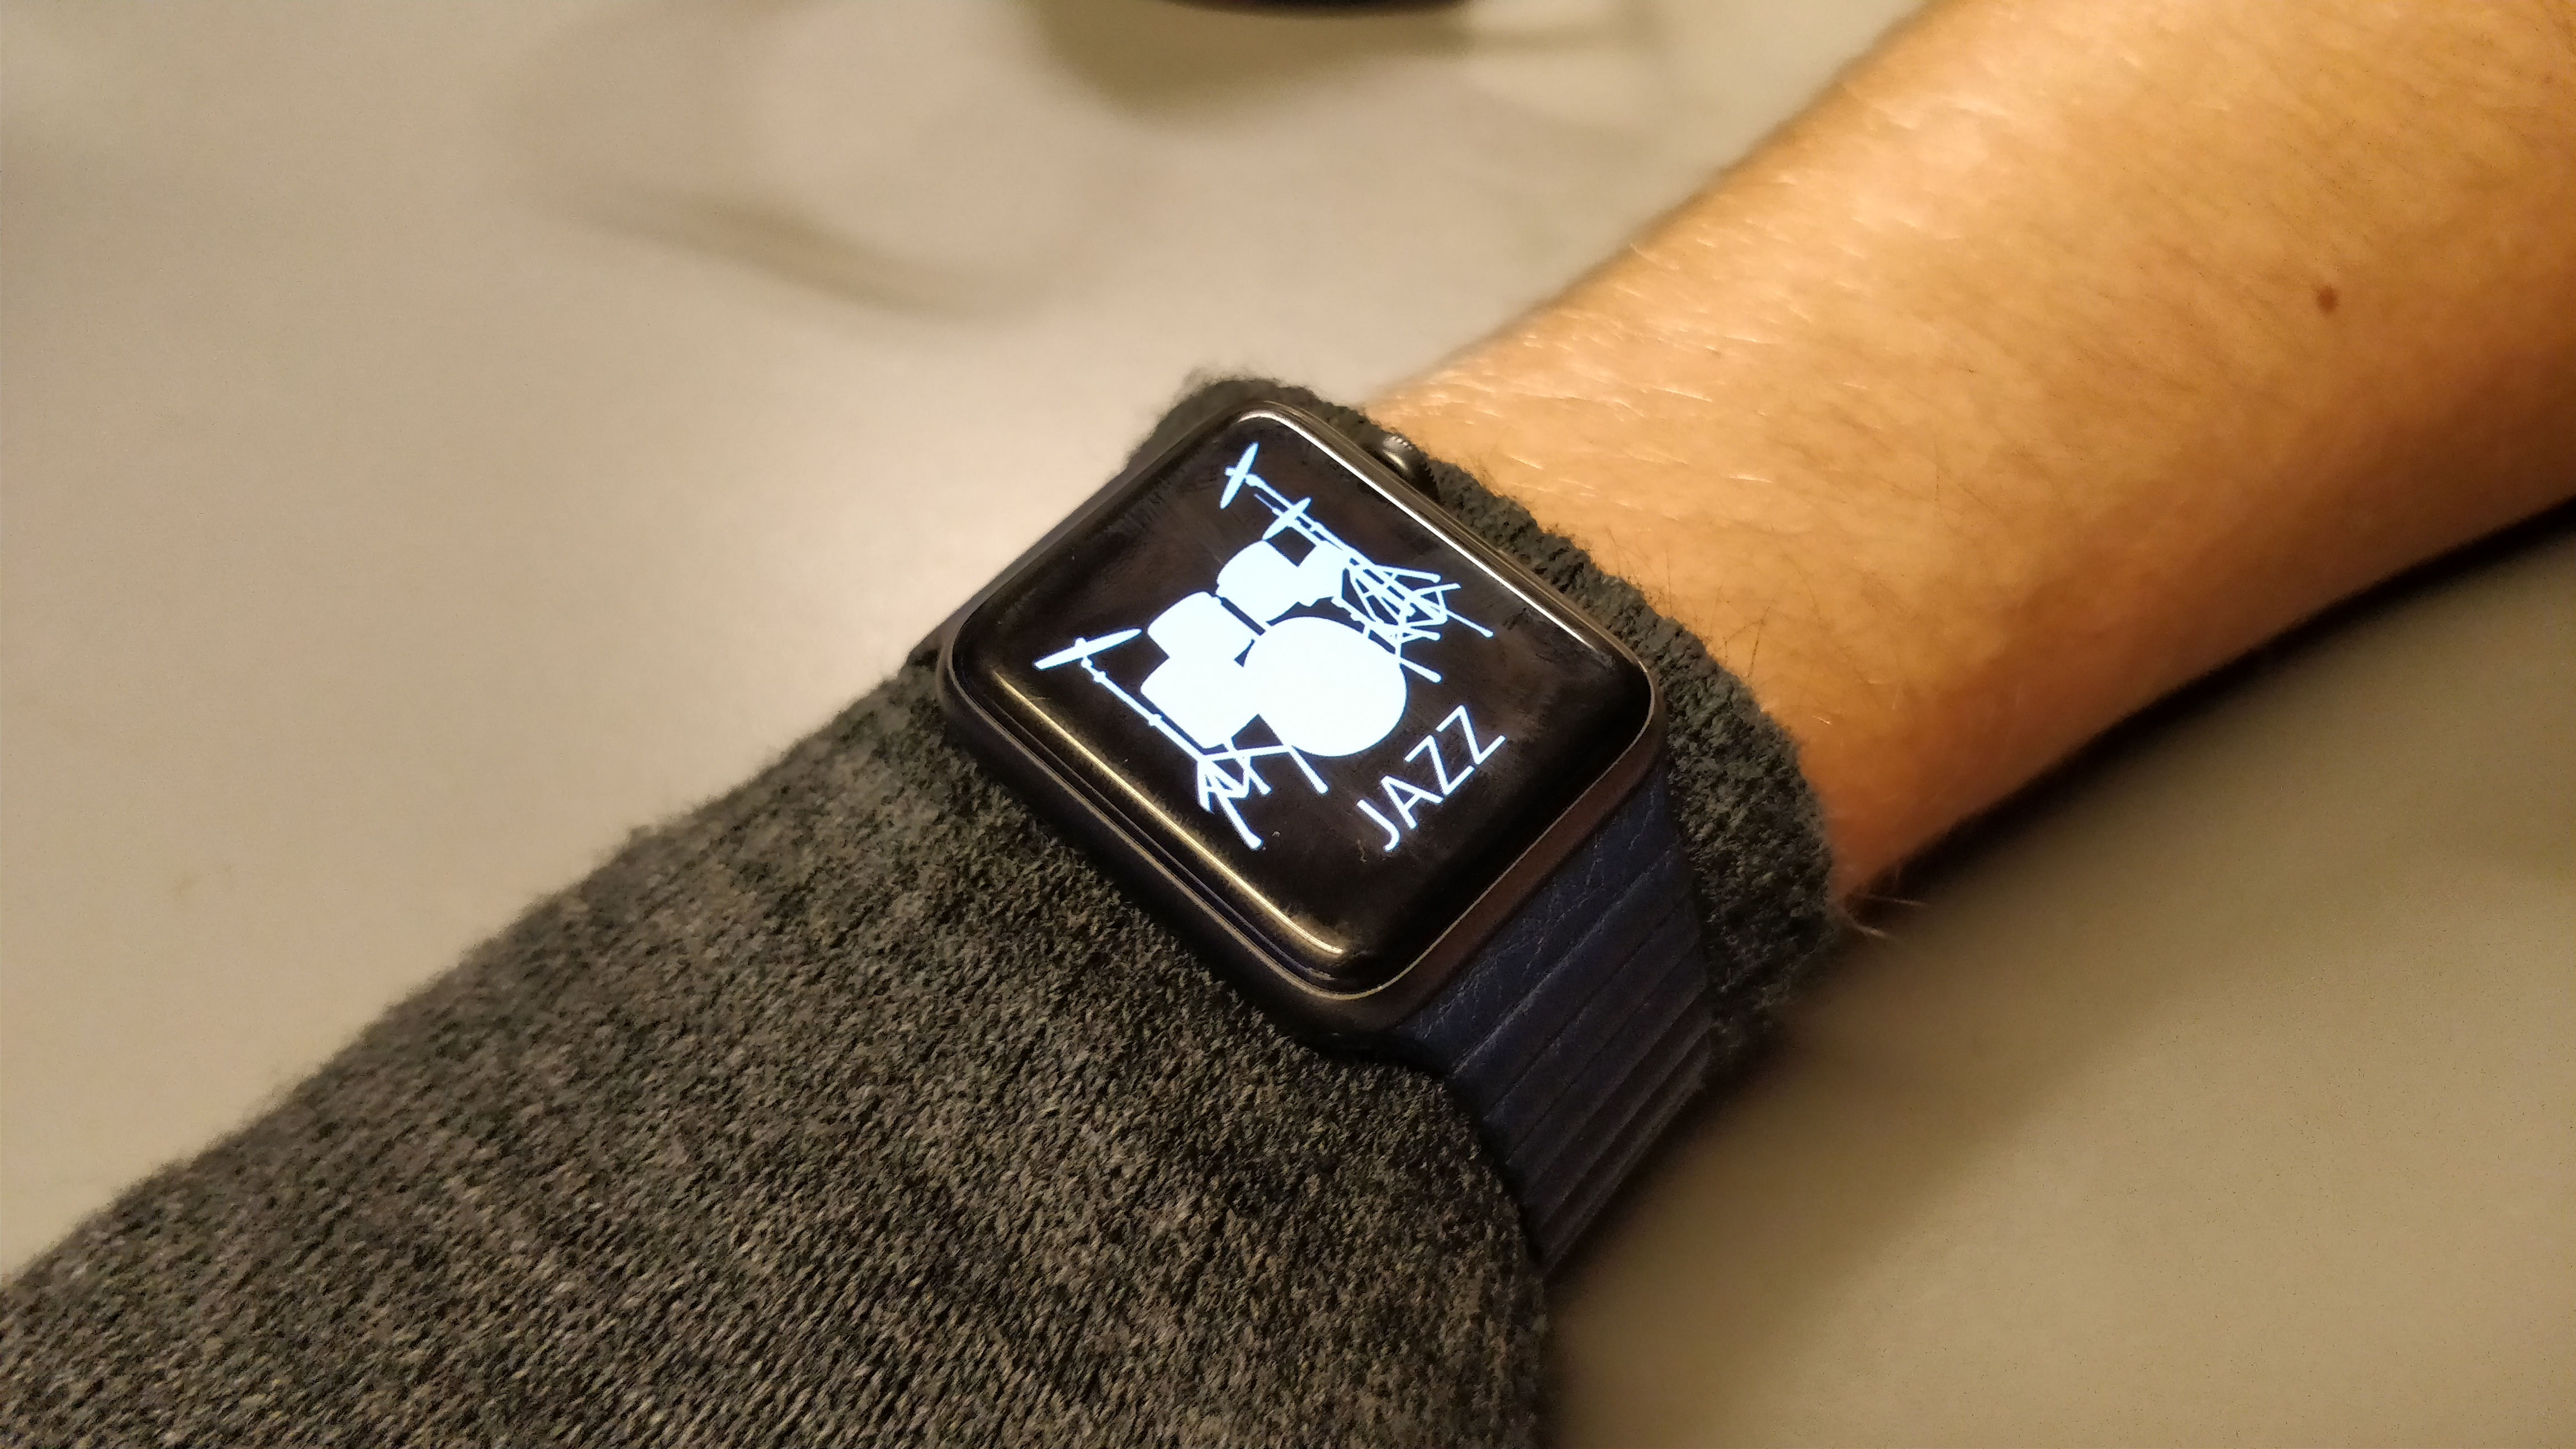
\includegraphics[scale=0.05]{Figure/Billeder/DisplayGlove.jpg}
\caption{A Future Vision of the FingerDrums glove with integrated display, storage etc. Shown here with an Apple Watch.}
\label{fig:DisplayGlove}
\end{figure}

Additionally, it would be nice to be able to record a beat and play it back later or even export it to audio editing software like Garageband. this would make FingerDrums a much more versatile tool and could make it useful for professional musicians and composers. 

\section{Midi Connectivity}
In order for the user to be able to easily change the drum sound profile it would make sense to work towards a MIDI configuration. Here the analogue signal from the FSR sensors needs to go through a AD converter and preferably to a device which also has either a WiFi or Bluetooth module built in. This way the digital signal is able to be sent to a MIDI software which translates the signal into the chosen sound. There are countless ways to expand the interactions possible so that the sounds are not only limited to playing drum sounds partly because we plan on using FSR sensors. Via MIDI it is possible to play whatever you like and the FSRs make it possible to vary the intensity of the sound in relation to how hard you press or even modulate pitch eg. if synthesised sounds are being played. As of now the prototype has a very small but noticable delay between being pushed and the sound being played. According to \parencite{Adelstein2003} the maximum delay in haptic to audio asynchrony is 24 ms. This means that the maximum delay between a person hitting a drum and noticing that the sound is delayed is 24 ms. In order to completely avoid having the user experience haptic to audio asynchrony it would be preferable to make it a requirement that the maximum allowable delay between the sensors transmitting the signal and the speakers playing the sound is 15 ms. This should be quite doable.

\section{Aesthetics }
The Aesthetics of the FingerDrums prototype are still at a very early stage and could stand to be updated. The first and simplest fix would be to cover up the wiring and sensors with a more neutral glove as in \autoref{fig:CoveredGlove} however if the changes mentioned above are implemented the wiring could be almost completely eliminated freeing up the glove for all kinds of unique and colorful designs.

\begin{figure}[H]
\centering
\includegraphics[scale=0.05]{Figure/Billeder/CoveredGlove.jpg}
\caption{The FingerDrums glove with sensors and some of the wiring covered.}
\label{fig:CoveredGlove}
\end{figure}

\section{Ergonomics}
Over the course of the development it was discovered that not all hands are created equal, and not everyone was able to use the FingerDrums glove without some modifications. The glove as it is is also somewhat thick and tight fitting resulting in a very hot glove that gets uncomfortable to wear after a short amount of time. As such thinner and more breathable and elastic fabric should be used and the sensors  positions made adjustable to better fit more different shapes and sizes of hands. 